\documentclass[10pt,a4paper]{article}
\usepackage{fontspec}
\defaultfontfeatures{Mapping=tex-text}
\usepackage{xunicode}
\usepackage{xltxtra}
%\setmainfont{???}
\usepackage{xeCJK}
\usepackage{ctex}
\usepackage{polyglossia}
\setdefaultlanguage{english}
\usepackage{indentfirst}
\setlength{\parindent}{2em}%中文缩进两个汉字位
\usepackage{amsmath}
\usepackage{amsfonts}
\usepackage{amssymb}
\usepackage{siunitx}


\usepackage{amsmath}
 \usepackage{siunitx}
\usepackage{geometry}

\author{翁俊}
\title{第十二周上机作业}

\begin{document}
\maketitle
\newpage
第一部分:当取的区间为[-1,1]时,其分布归一化后为:
\[
f(x)=\frac{3}{2\times (3+\beta)}(1+\alpha x+\beta x^2)
\]

最终的拟合结果如图:
\begin{figure}[ht]
 \centering
 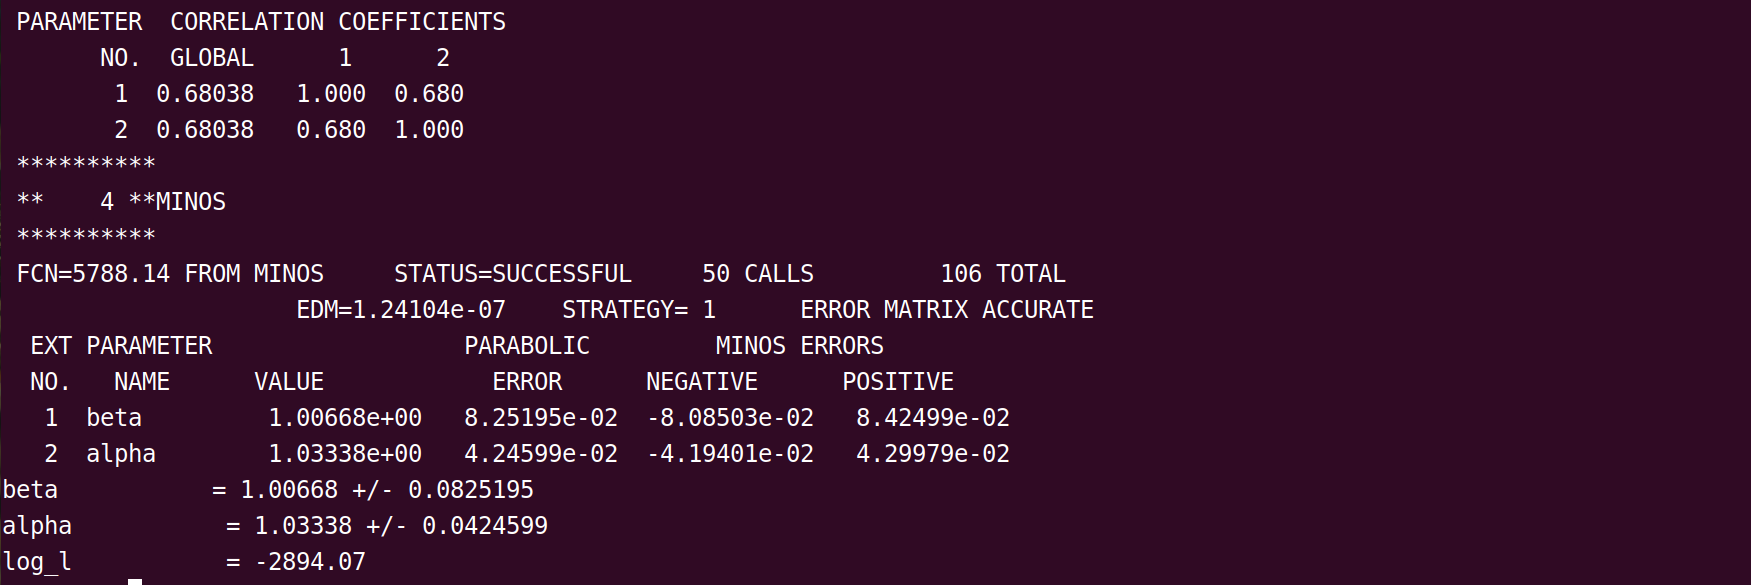
\includegraphics[height=5cm]{img/wj1.png}
 \caption{区间为[-1,1]时的拟合结果}
 \label{fig:singleblock}
\end{figure}

\newpage
第二部分:当取的区间为[-0.95,0.95]时,其分布归一化后为:
\[
f(x)=\frac{3}{5.7+2\times \beta \times 0.95^3}(1+\alpha x+\beta x^2)
\]

最终的拟合结果如图:
\begin{figure}[ht]
 \centering
 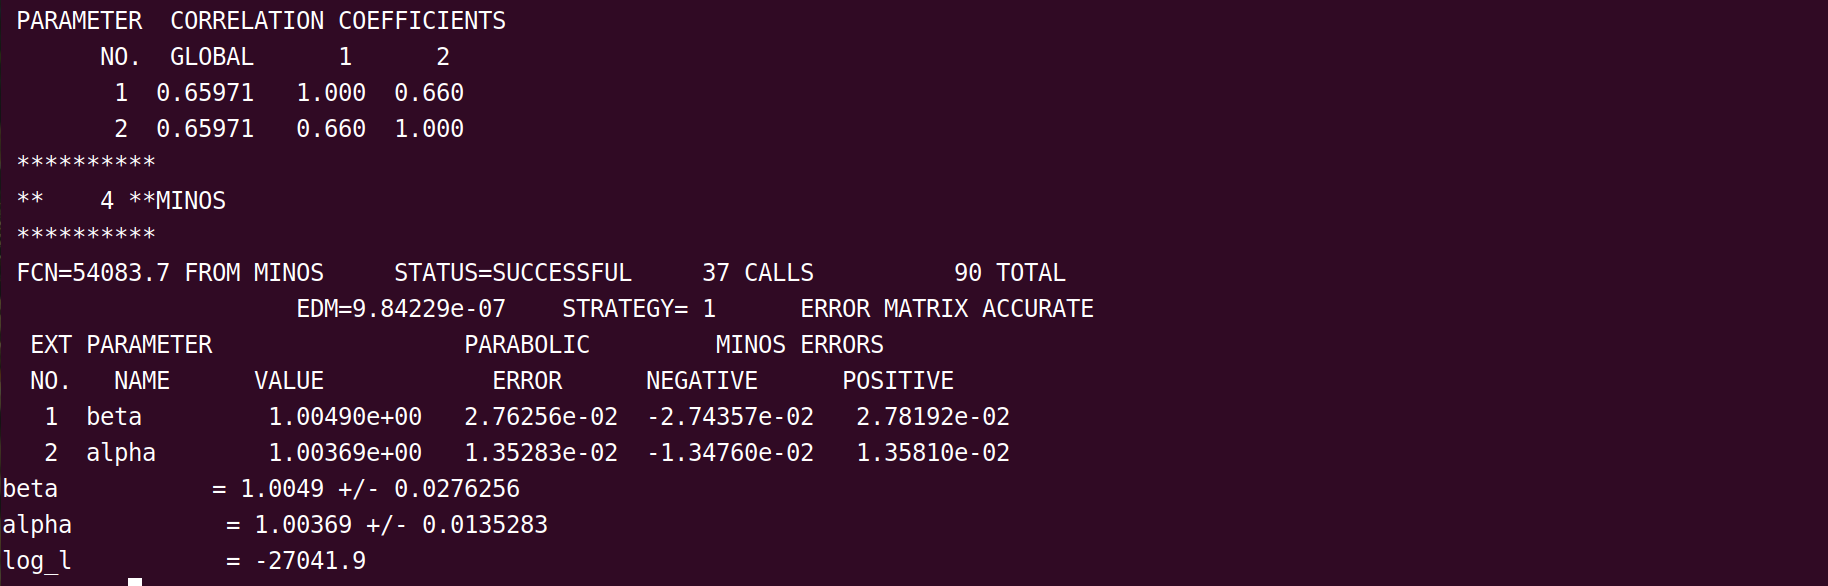
\includegraphics[height=5cm]{img/wj2.png}
 \caption{区间为[-0.95,0.95]时的拟合结果}
 \label{fig:singleblock}
\end{figure}

\end{document}